% Options for packages loaded elsewhere
\PassOptionsToPackage{unicode}{hyperref}
\PassOptionsToPackage{hyphens}{url}
%
\documentclass[
  a4paper,
]{article}
\usepackage{amsmath,amssymb}
\usepackage{iftex}
\ifPDFTeX
  \usepackage[T1]{fontenc}
  \usepackage[utf8]{inputenc}
  \usepackage{textcomp} % provide euro and other symbols
\else % if luatex or xetex
  \usepackage{unicode-math} % this also loads fontspec
  \defaultfontfeatures{Scale=MatchLowercase}
  \defaultfontfeatures[\rmfamily]{Ligatures=TeX,Scale=1}
\fi
\usepackage{lmodern}
\ifPDFTeX\else
  % xetex/luatex font selection
    \setmainfont[]{Helvetica}
\fi
% Use upquote if available, for straight quotes in verbatim environments
\IfFileExists{upquote.sty}{\usepackage{upquote}}{}
\IfFileExists{microtype.sty}{% use microtype if available
  \usepackage[]{microtype}
  \UseMicrotypeSet[protrusion]{basicmath} % disable protrusion for tt fonts
}{}
\makeatletter
\@ifundefined{KOMAClassName}{% if non-KOMA class
  \IfFileExists{parskip.sty}{%
    \usepackage{parskip}
  }{% else
    \setlength{\parindent}{0pt}
    \setlength{\parskip}{6pt plus 2pt minus 1pt}}
}{% if KOMA class
  \KOMAoptions{parskip=half}}
\makeatother
\usepackage{xcolor}
\usepackage[margin=0.75in]{geometry}
\usepackage{graphicx}
\makeatletter
\newsavebox\pandoc@box
\newcommand*\pandocbounded[1]{% scales image to fit in text height/width
  \sbox\pandoc@box{#1}%
  \Gscale@div\@tempa{\textheight}{\dimexpr\ht\pandoc@box+\dp\pandoc@box\relax}%
  \Gscale@div\@tempb{\linewidth}{\wd\pandoc@box}%
  \ifdim\@tempb\p@<\@tempa\p@\let\@tempa\@tempb\fi% select the smaller of both
  \ifdim\@tempa\p@<\p@\scalebox{\@tempa}{\usebox\pandoc@box}%
  \else\usebox{\pandoc@box}%
  \fi%
}
% Set default figure placement to htbp
\def\fps@figure{htbp}
\makeatother
\setlength{\emergencystretch}{3em} % prevent overfull lines
\providecommand{\tightlist}{%
  \setlength{\itemsep}{0pt}\setlength{\parskip}{0pt}}
\setcounter{secnumdepth}{-\maxdimen} % remove section numbering
\usepackage{titling}
\pretitle{\begin{flushleft}}
\posttitle{\end{flushleft}}
\usepackage{booktabs}
\usepackage{longtable}
\usepackage{float}
\floatplacement{figure}{H}
\usepackage{colortbl}
\usepackage{pdflscape}
\usepackage{tabu}
\usepackage{makecell}
\usepackage{xcolor}
\usepackage{soul}
\usepackage{caption}
\usepackage[singlelinecheck=false]{caption}
\usepackage[font={small,bf}]{caption}
\usepackage{multirow}
\usepackage{array}
\usepackage{lscape}
\newcommand{\blandscape}{\begin{landscape}}
\newcommand{\elandscape}{\end{landscape}}
\usepackage[dvipsnames]{xcolor}
\renewcommand{\footnotesize}{\tiny}
\usepackage{threeparttable}
\usepackage{bookmark}
\IfFileExists{xurl.sty}{\usepackage{xurl}}{} % add URL line breaks if available
\urlstyle{same}
\hypersetup{
  hidelinks,
  pdfcreator={LaTeX via pandoc}}

\title{\vspace{-1.5cm} \begin{LARGE} WGS Quality Control Report \end{LARGE}}
\author{}
\date{\vspace{-2.5em}}

\begin{document}
\maketitle

\normalsize Batch Name: 2025-07-08\_P

\normalsize Experiment Name: 25ARS\_UTP\_SSR\_LY9CL

\fontsize{7}{8}
\selectfont
\captionsetup[table]{labelformat=empty}
\renewcommand{\arraystretch}{1.2}

\begin{tabular}{>{\centering\arraybackslash}p{1cm}>{\centering\arraybackslash}p{2.8cm}>{\centering\arraybackslash}p{1.5cm}>{\centering\arraybackslash}p{5cm}>{\centering\arraybackslash}p{5cm}}
\toprule
\multicolumn{1}{>{\centering\arraybackslash}p{1cm}}{\cellcolor[HTML]{D4D4D4}{\textbf{Isolate No.}}} & \multicolumn{1}{>{\centering\arraybackslash}p{2.8cm}}{\cellcolor[HTML]{D4D4D4}{\textbf{Sample ID}}} & \multicolumn{1}{>{\centering\arraybackslash}p{1.5cm}}{\cellcolor[HTML]{D4D4D4}{\textbf{Description}}} & \multicolumn{1}{>{\centering\arraybackslash}p{5cm}}{\cellcolor[HTML]{D4D4D4}{\textbf{ARSRL}}} & \multicolumn{1}{>{\centering\arraybackslash}p{5cm}}{\cellcolor[HTML]{D4D4D4}{\textbf{WGS}}}\\
\midrule
1 & 25ARS\_MAR0011 & UDI165 & \em{Escherichia coli} & \em{Escherichia coli}\\
2 & UTPN\_BL\_016 & UDI174 & \em{Escherichia coli} & \em{Escherichia coli}\\
3 & UTPN\_BL\_017 & UDI175 & \em{Escherichia coli} & \em{Escherichia coli}\\
4 & UTPR\_BL\_002 & UDI170 & \em{Escherichia coli} & \em{Escherichia coli}\\
5 & UTPR\_BL\_003 & UDI171 & \em{Escherichia coli} & \em{Escherichia coli}\\
\addlinespace
6 & UTPR\_BL\_005 & UDI173 & \em{Escherichia coli} & \em{Escherichia coli}\\
7 & UTPR\_ST\_148 & UDI178 & \em{Escherichia coli} & \em{Escherichia coli}\\
8 & UTPR\_ST\_182 & UDI179 & \em{Escherichia coli} & \em{Escherichia coli}\\
9 & UTPR\_ST\_189 & UDI180 & \em{Escherichia coli} & \em{Escherichia coli}\\
\cellcolor[HTML]{FD7979}{10} & \cellcolor[HTML]{FD7979}{25ARS\_BGH0044} & \cellcolor[HTML]{FD7979}{UDI181} & \cellcolor[HTML]{FD7979}{\em{Klebsiella pneumoniae}} & \cellcolor[HTML]{FD7979}{\em{Klebsiella pneumoniae}}\\
\addlinespace
11 & 25ARS\_CRH0014 & UDI159 & \em{Klebsiella pneumoniae} & \em{Klebsiella pneumoniae}\\
12 & 25ARS\_CRH0015 & UDI160 & \em{Klebsiella pneumoniae} & \em{Klebsiella pneumoniae}\\
13 & 25ARS\_STU0019 & UDI190 & \em{Klebsiella pneumoniae} & \em{Klebsiella pneumoniae}\\
14 & 25ARS\_MMH0019 & UDI158 & \em{Klebsiella pneumoniae} & \em{Klebsiella pneumoniae}\\
15 & 25ARS\_RMC0008 & UDI098 & \em{Klebsiella pneumoniae} & \em{Klebsiella pneumoniae}\\
\addlinespace
16 & 25ARS\_RMC0009 & UDI099 & \em{Klebsiella pneumoniae} & \em{Klebsiella pneumoniae}\\
17 & 25ARS\_STU0020 & UDI191 & \em{Klebsiella pneumoniae} & \em{Klebsiella pneumoniae}\\
18 & 25ARS\_ZMC0007 & UDI103 & \em{Klebsiella pneumoniae} & \em{Klebsiella pneumoniae}\\
19 & 24ARS\_MAR0196 & UDI163 & \em{Pseudomonas aeruginosa} & \em{Pseudomonas aeruginosa}\\
\bottomrule
\multicolumn{5}{l}{\rule{0pt}{1em}\textit{Legend:} PASS   |   \colorbox{Salmon}{FAILURE}   |   \textcolor{Blue}{EXCEEDS THRESHOLD METRIC/S}   |   (x) - NON-CONCORDANT   |}\\
\end{tabular}

\fontsize{7}{8}
\selectfont
\captionsetup[table]{labelformat=empty}
\renewcommand{\arraystretch}{1.2}

\(\\\) \newpage

\begin{landscape}
\fontsize{7}{8}
\selectfont
\captionsetup[table]{labelformat=empty}
\renewcommand{\arraystretch}{1.2}

\begin{table}[!h]
\centering
\resizebox{\ifdim\width>\linewidth\linewidth\else\width\fi}{!}{
\begin{tabular}{cc>{}ccccccccc}
\toprule
\cellcolor[HTML]{D4D4D4}{\textbf{Isolate No.}} & \cellcolor[HTML]{D4D4D4}{\textbf{Sample ID}} & \cellcolor[HTML]{D4D4D4}{\textbf{WGS ID}} & \cellcolor[HTML]{D4D4D4}{\textbf{completeness}} & \cellcolor[HTML]{D4D4D4}{\textbf{contamination}} & \cellcolor[HTML]{D4D4D4}{\textbf{Depth of coverage}} & \cellcolor[HTML]{D4D4D4}{\textbf{Genome size}} & \cellcolor[HTML]{D4D4D4}{\textbf{GC content}} & \cellcolor[HTML]{D4D4D4}{\textbf{Contig count}} & \cellcolor[HTML]{D4D4D4}{\textbf{N50}} & \cellcolor[HTML]{D4D4D4}{\textbf{Mean read Q-score}}\\
\midrule
1 & 25ARS\_MAR0011 & \em{Escherichia coli} & 100 & 0.11 & 81.8 & 4.98 Mb & 50.82 & 119 & 117099 & 36.9\\
2 & UTPN\_BL\_016 & \em{Escherichia coli} & 100 & 0.13 & 37.6 & 4.93 Mb & 50.5 & 107 & 113278 & 36.7\\
3 & UTPN\_BL\_017 & \em{Escherichia coli} & 100 & 0.48 & 25.0 & 4.95 Mb & 50.73 & 186 & 89194 & 36.8\\
4 & UTPR\_BL\_002 & \em{Escherichia coli} & 100 & 0.16 & 52.4 & 4.93 Mb & 50.62 & 64 & 215097 & 36.5\\
5 & UTPR\_BL\_003 & \em{Escherichia coli} & 100 & 0.79 & 60.4 & 4.92 Mb & 50.76 & 98 & 239857 & 36.9\\
\addlinespace
6 & UTPR\_BL\_005 & \em{Escherichia coli} & 100 & 0.52 & 38.4 & 5.05 Mb & 50.63 & 88 & 317164 & 36.7\\
7 & UTPR\_ST\_148 & \em{Escherichia coli} & 100 & 0.13 & 47.0 & 4.89 Mb & 50.64 & 66 & 211593 & 36.8\\
8 & UTPR\_ST\_182 & \em{Escherichia coli} & 100 & 0.23 & 60.6 & 5.19 Mb & 50.61 & 159 & 111647 & 37.0\\
9 & UTPR\_ST\_189 & \em{Escherichia coli} & 100 & 0.15 & 44.0 & 4.73 Mb & 50.88 & 80 & 169011 & 36.8\\
\cellcolor[HTML]{FD7979}{10} & \cellcolor[HTML]{FD7979}{25ARS\_BGH0044} & \em{\cellcolor[HTML]{FD7979}{Klebsiella pneumoniae}} & \cellcolor[HTML]{FD7979}{100} & \cellcolor[HTML]{FD7979}{1} & \cellcolor[HTML]{FD7979}{\textcolor{blue}{\textbf{19.8}}} & \cellcolor[HTML]{FD7979}{5.73 Mb} & \cellcolor[HTML]{FD7979}{57.1} & \cellcolor[HTML]{FD7979}{85} & \cellcolor[HTML]{FD7979}{178089} & \cellcolor[HTML]{FD7979}{36.5}\\
\addlinespace
11 & 25ARS\_CRH0014 & \em{Klebsiella pneumoniae} & 100 & 0.12 & 33.7 & 5.58 Mb & 57.04 & 84 & 214908 & 36.7\\
12 & 25ARS\_CRH0015 & \em{Klebsiella pneumoniae} & 100 & 0.12 & 39.8 & 5.31 Mb & 57.36 & 107 & 157575 & 36.7\\
13 & 25ARS\_STU0019 & \em{Klebsiella pneumoniae} & 100 & 0.51 & 54.1 & 5.49 Mb & 57.13 & 70 & 296147 & 36.6\\
14 & 25ARS\_MMH0019 & \em{Klebsiella pneumoniae} & 100 & 0.12 & 46.9 & 5.69 Mb & 56.91 & 94 & 260143 & 36.5\\
15 & 25ARS\_RMC0008 & \em{Klebsiella pneumoniae} & 100 & 0.41 & 62.6 & 5.77 Mb & 56.97 & 124 & 254414 & 36.7\\
\addlinespace
16 & 25ARS\_RMC0009 & \em{Klebsiella pneumoniae} & 100 & 0.84 & 57.0 & 5.75 Mb & 56.59 & 70 & 275489 & 36.7\\
17 & 25ARS\_STU0020 & \em{Klebsiella pneumoniae} & 100 & 0.24 & 62.0 & 5.44 Mb & 57.3 & 72 & 215906 & 36.6\\
18 & 25ARS\_ZMC0007 & \em{Klebsiella pneumoniae} & 100 & 0.66 & 32.8 & 5.70 Mb & 57.04 & 128 & 262125 & 36.6\\
19 & 24ARS\_MAR0196 & \em{Pseudomonas aeruginosa} & 100 & 0.07 & 34.3 & 6.26 Mb & 66.56 & 53 & 477553 & 36.2\\
20 & 24ARS\_MAR227 & \em{Pseudomonas aeruginosa} & 100 & 0.05 & 68.9 & 7.45 Mb & 65.35 & 141 & 176111 & 36.1\\
\bottomrule
\multicolumn{11}{l}{\rule{0pt}{1em}\textit{Legend:} PASS   |   \colorbox{Salmon}{FAILURE}   |   \textcolor{Blue}{EXCEEDS THRESHOLD METRIC/S}   |   (x) - NON-CONCORDANT   |}\\
\end{tabular}}
\end{table}









$\\$ $\\$ $\\$ $\color{red}{\normalsize\textbf{RECOMMENDATION:}}$



\begin{tabular}{>{\raggedright\arraybackslash}p{6cm}>{\centering\arraybackslash}p{6cm}>{\centering\arraybackslash}p{4cm}}
\toprule
\cellcolor[HTML]{D4D4D4}{\textbf{Sample ID}} & \cellcolor[HTML]{D4D4D4}{\textbf{Reason - Failed Metrics}} & \cellcolor[HTML]{D4D4D4}{\textbf{Remarks}}\\
\midrule
\cellcolor{gray!10}{25ARS\_BGH0044} & \cellcolor{gray!10}{Depth of coverage} & \cellcolor{gray!10}{For repeat testing}\\
\bottomrule
\end{tabular}



\end{landscape}

\fontsize{7}{8}
\selectfont
\captionsetup[table]{labelformat=empty}
\renewcommand{\arraystretch}{1.2}

\begin{tabular}{>{\raggedright\arraybackslash}p{8cm}c}
\toprule
\cellcolor[HTML]{D4D4D4}{\textbf{WGS\_ID}} & \cellcolor[HTML]{D4D4D4}{\textbf{Number}}\\
\midrule
\em{Escherichia coli} & 9\\
\em{Klebsiella pneumoniae} & 9\\
\em{Pseudomonas aeruginosa} & 1\\
\bottomrule
\end{tabular}

\begin{itemize}
\item
  \(\color{red}3\) distinct species were identified among
  \(\color{red}19\) isolates.
\item
  \(\color{red}100.00\) \% (n=19) of the isolates passed the QC, while
  \(\color{red}5.26\) \% (n=1) were tagged with failure.
\item
  Concordance between ARSRL and WGS species report was
  \(\color{red}100.00\) \%. \(\\\)
\end{itemize}

\subsubsection{GRAPHS}\label{graphs}

\fontsize{7}{8}
\selectfont
\captionsetup[table]{labelformat=empty}
\renewcommand{\arraystretch}{1.2}

\pandocbounded{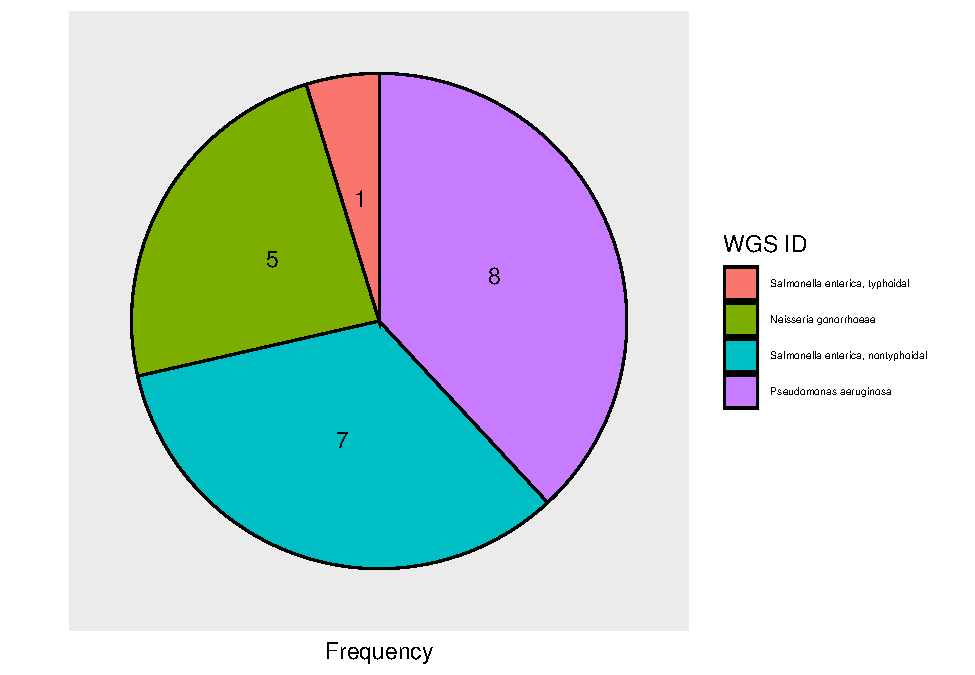
\includegraphics[keepaspectratio]{ARSRL_WGS_QC_report_2025-07-08_P_files/figure-latex/pie_chart-1.pdf}}

\subsubsection{Result Classification}\label{result-classification}

\pandocbounded{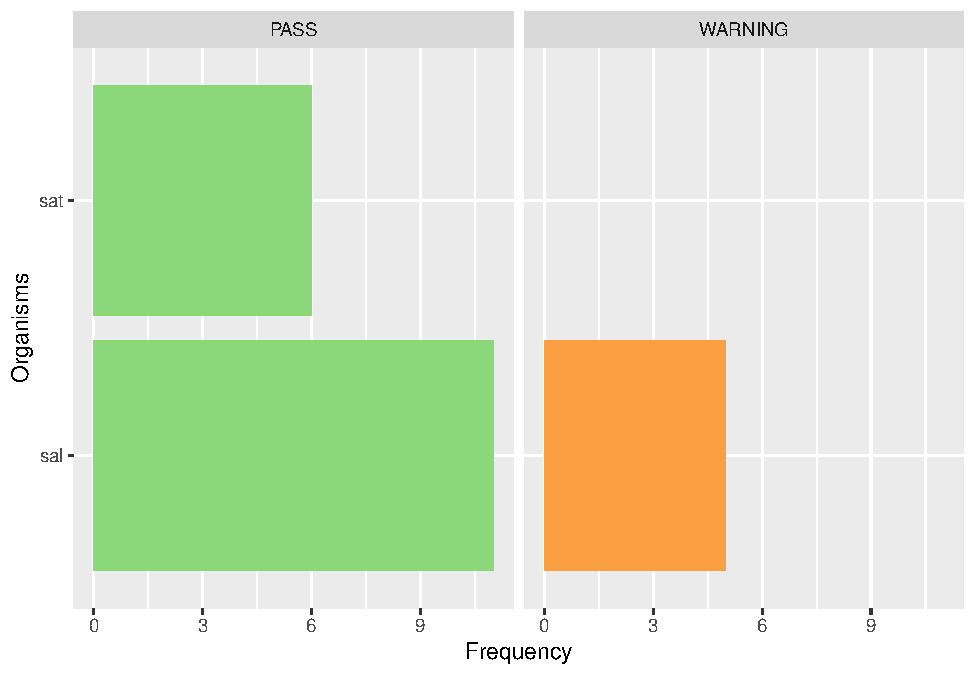
\includegraphics[keepaspectratio]{ARSRL_WGS_QC_report_2025-07-08_P_files/figure-latex/organism results-1.pdf}}

\subsubsection{Number of contigs}\label{number-of-contigs}

\pandocbounded{\includegraphics[keepaspectratio]{ARSRL_WGS_QC_report_2025-07-08_P_files/figure-latex/contigs_result-1.pdf}}

\subsubsection{N50 Value}\label{n50-value}

\pandocbounded{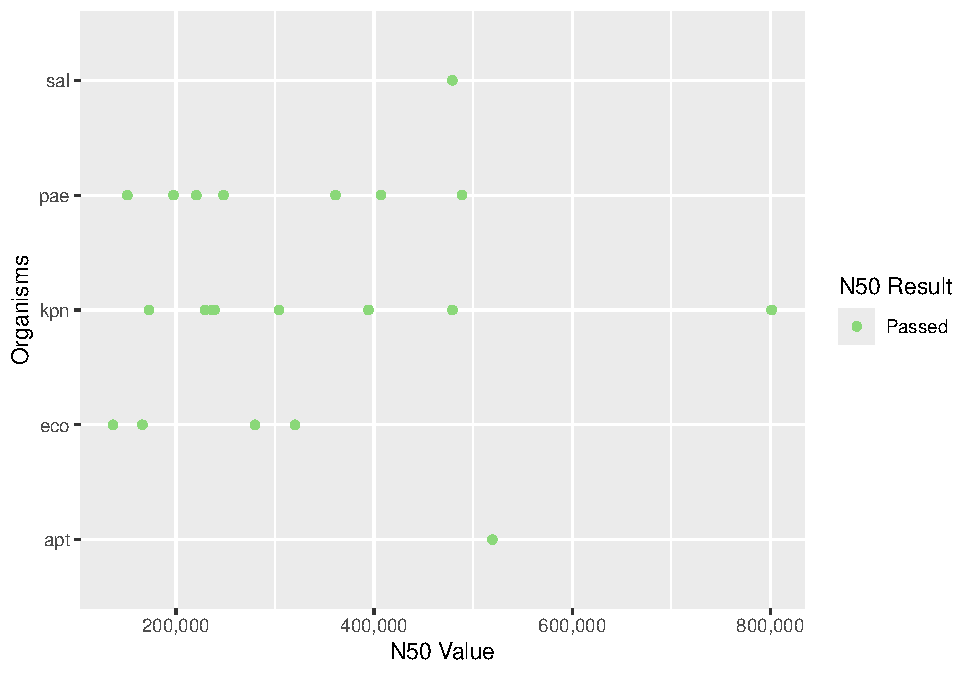
\includegraphics[keepaspectratio]{ARSRL_WGS_QC_report_2025-07-08_P_files/figure-latex/n50_result -1.pdf}}

\subsubsection{Total Length}\label{total-length}

\pandocbounded{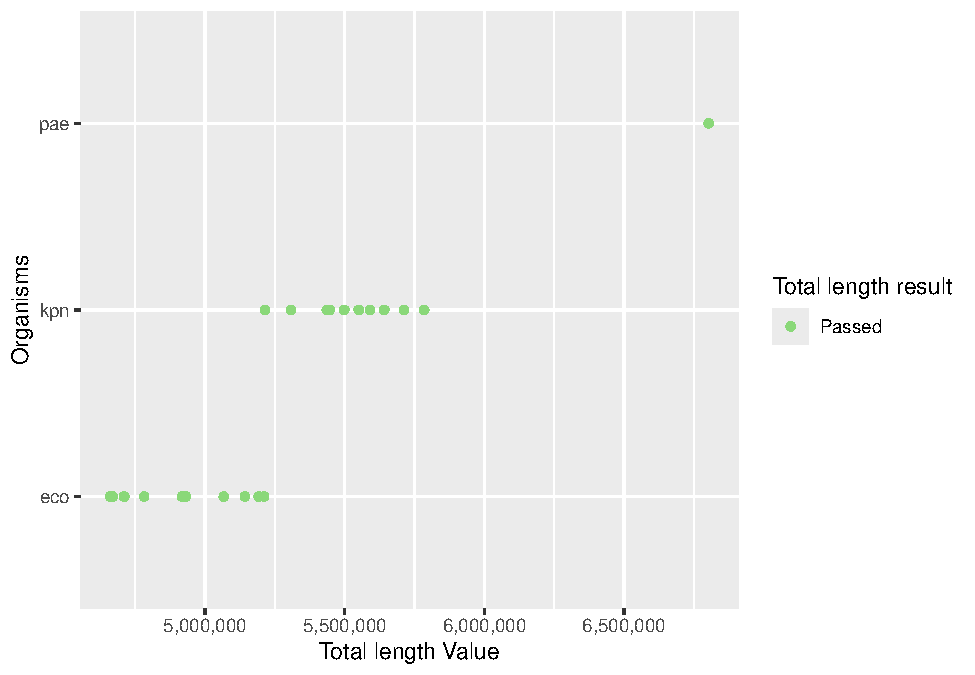
\includegraphics[keepaspectratio]{ARSRL_WGS_QC_report_2025-07-08_P_files/figure-latex/length_result -1.pdf}}

\fontsize{7}{8}
\selectfont
\captionsetup[table]{labelformat=empty}
\renewcommand{\arraystretch}{1}

\subsubsection{MLST RESULTS}\label{mlst-results}

\resizebox{\ifdim\width>\linewidth\linewidth\else\width\fi}{!}{
\begin{tabular}{>{\centering\arraybackslash}p{3cm}>{\centering\arraybackslash}p{3cm}>{\centering\arraybackslash}p{1cm}>{\centering\arraybackslash}p{1cm}>{\centering\arraybackslash}p{1cm}>{\centering\arraybackslash}p{1cm}>{\centering\arraybackslash}p{1cm}>{\centering\arraybackslash}p{1cm}>{\centering\arraybackslash}p{1cm}>{\centering\arraybackslash}p{1cm}}
\toprule
\cellcolor[HTML]{D4D4D4}{\textbf{sample\_id}} & \cellcolor[HTML]{D4D4D4}{\textbf{species}} & \cellcolor[HTML]{D4D4D4}{\textbf{MLST}} & \cellcolor[HTML]{D4D4D4}{\textbf{acsA}} & \cellcolor[HTML]{D4D4D4}{\textbf{aroE}} & \cellcolor[HTML]{D4D4D4}{\textbf{guaA}} & \cellcolor[HTML]{D4D4D4}{\textbf{mutL}} & \cellcolor[HTML]{D4D4D4}{\textbf{nuoD}} & \cellcolor[HTML]{D4D4D4}{\textbf{ppsA}} & \cellcolor[HTML]{D4D4D4}{\textbf{trpE}}\\
\midrule
24ARS\_MAR0196 & \em{Pseudomonas aeruginosa} & 645 & 6 & 5 & 5 & 3 & 3 & 13 & 1\\
24ARS\_MAR227 & \em{Pseudomonas aeruginosa} & 773 & 5 & 4 & 5 & 5 & 5 & 7 & 8\\
\bottomrule
\multicolumn{10}{l}{\rule{0pt}{1em}\textit{Legend: } (-) Not identified}\\
\end{tabular}}

\resizebox{\ifdim\width>\linewidth\linewidth\else\width\fi}{!}{
\begin{tabular}{>{\centering\arraybackslash}p{3cm}>{\centering\arraybackslash}p{3cm}>{\centering\arraybackslash}p{1cm}>{\centering\arraybackslash}p{1cm}>{\centering\arraybackslash}p{1cm}>{\centering\arraybackslash}p{1cm}>{\centering\arraybackslash}p{1cm}>{\centering\arraybackslash}p{1cm}>{\centering\arraybackslash}p{1cm}>{\centering\arraybackslash}p{1cm}}
\toprule
\cellcolor[HTML]{D4D4D4}{\textbf{sample\_id}} & \cellcolor[HTML]{D4D4D4}{\textbf{species}} & \cellcolor[HTML]{D4D4D4}{\textbf{MLST}} & \cellcolor[HTML]{D4D4D4}{\textbf{acsA}} & \cellcolor[HTML]{D4D4D4}{\textbf{aroE}} & \cellcolor[HTML]{D4D4D4}{\textbf{guaA}} & \cellcolor[HTML]{D4D4D4}{\textbf{mutL}} & \cellcolor[HTML]{D4D4D4}{\textbf{nuoD}} & \cellcolor[HTML]{D4D4D4}{\textbf{ppsA}} & \cellcolor[HTML]{D4D4D4}{\textbf{trpE}}\\
\midrule
25ARS\_BGH0044 & \em{Klebsiella pneumoniae} & 23 & 2 & 1 & 1 & 1 & 9 & 4 & 12\\
25ARS\_CRH0014 & \em{Klebsiella pneumoniae} & 101 & 2 & 6 & 1 & 5 & 4 & 1 & 6\\
25ARS\_CRH0015 & \em{Klebsiella pneumoniae} & 3140 & 2 & 5 & 1 & 1 & 1 & 4 & 9\\
25ARS\_MMH0019 & \em{Klebsiella pneumoniae} & 231 & 2 & 6 & 1 & 3 & 26 & 1 & 77\\
25ARS\_RMC0008 & \em{Klebsiella pneumoniae} & 515 & 2 & 1 & 1 & 1 & 1 & 1 & 4\\
\addlinespace
25ARS\_RMC0009 & \em{Klebsiella pneumoniae} & 309 & 2 & 9 & 2 & 1 & 13 & 1 & 10\\
25ARS\_STU0019 & \em{Klebsiella pneumoniae} & 101 & 2 & 6 & 1 & 5 & 4 & 1 & 6\\
25ARS\_STU0020 & \em{Klebsiella pneumoniae} & 307 & 4 & 1 & 2 & 52 & 1 & 1 & 7\\
25ARS\_ZMC0007 & \em{Klebsiella pneumoniae} & 45 & 2 & 1 & 1 & 6 & 7 & 1 & 12\\
\bottomrule
\multicolumn{10}{l}{\rule{0pt}{1em}\textit{Legend: } (-) Not identified}\\
\end{tabular}}

\resizebox{\ifdim\width>\linewidth\linewidth\else\width\fi}{!}{
\begin{tabular}{>{\centering\arraybackslash}p{3cm}>{\centering\arraybackslash}p{3cm}>{\centering\arraybackslash}p{1cm}>{\centering\arraybackslash}p{1cm}>{\centering\arraybackslash}p{1cm}>{\centering\arraybackslash}p{1cm}>{\centering\arraybackslash}p{1cm}>{\centering\arraybackslash}p{1cm}>{\centering\arraybackslash}p{1cm}>{\centering\arraybackslash}p{1cm}}
\toprule
\cellcolor[HTML]{D4D4D4}{\textbf{sample\_id}} & \cellcolor[HTML]{D4D4D4}{\textbf{species}} & \cellcolor[HTML]{D4D4D4}{\textbf{MLST}} & \cellcolor[HTML]{D4D4D4}{\textbf{acsA}} & \cellcolor[HTML]{D4D4D4}{\textbf{aroE}} & \cellcolor[HTML]{D4D4D4}{\textbf{guaA}} & \cellcolor[HTML]{D4D4D4}{\textbf{mutL}} & \cellcolor[HTML]{D4D4D4}{\textbf{nuoD}} & \cellcolor[HTML]{D4D4D4}{\textbf{ppsA}} & \cellcolor[HTML]{D4D4D4}{\textbf{trpE}}\\
\midrule
25ARS\_MAR0011 & \em{Escherichia coli} & 361 & 10 & 99 & 5 & 91 & 8 & 7 & 2\\
UTPN\_BL\_016 & \em{Escherichia coli} & 410 & 6 & 4 & 12 & 1 & 20 & 18 & 7\\
UTPN\_BL\_017 & \em{Escherichia coli} & 44 & 10 & 11 & 4 & 8 & 8 & 8 & 7\\
UTPR\_BL\_002 & \em{Escherichia coli} & 58 & 6 & 4 & 4 & 16 & 24 & 8 & 14\\
UTPR\_BL\_003 & \em{Escherichia coli} & 131 & 53 & 40 & 47 & 13 & 36 & 28 & 29\\
\addlinespace
UTPR\_BL\_005 & \em{Escherichia coli} & 144 & 13 & 43 & 9 & 36 & 30 & 44 & 25\\
UTPR\_ST\_148 & \em{Escherichia coli} & 1722 & 101 & 4 & 97 & 29 & 70 & 158 & 2\\
UTPR\_ST\_182 & \em{Escherichia coli} & 155 & 6 & 4 & 14 & 16 & 24 & 8 & 14\\
UTPR\_ST\_189 & \em{Escherichia coli} & 1431 & 6 & 65 & 3 & 1 & 11 & 13 & 6\\
\bottomrule
\multicolumn{10}{l}{\rule{0pt}{1em}\textit{Legend: } (-) Not identified}\\
\end{tabular}}

\subsubsection{MLST RESULTS SUMMARY:}\label{mlst-results-summary}

\begin{tabular}{>{\raggedright\arraybackslash}p{6cm}>{\raggedright\arraybackslash}p{10cm}}
\toprule
\cellcolor[HTML]{D4D4D4}{\textbf{wgs\_id}} & \cellcolor[HTML]{D4D4D4}{\textbf{mlst\_count}}\\
\midrule
\em{Pseudomonas aeruginosa} & 645 (n= 1 ), 773 (n= 1 )\\
\em{Klebsiella pneumoniae} & 23 (n= 1 ), 101 (n= 2 ), 3140 (n= 1 ), 231 (n= 1 ), 515 (n= 1 ), 309 (n= 1 ), 307 (n= 1 ), 45 (n= 1 )\\
\em{Escherichia coli} & 361 (n= 1 ), 410 (n= 1 ), 44 (n= 1 ), 58 (n= 1 ), 131 (n= 1 ), 144 (n= 1 ), 1722 (n= 1 ), 155 (n= 1 ), 1431 (n= 1 )\\
\bottomrule
\multicolumn{2}{l}{\rule{0pt}{1em}\textit{Legend: } (-) Not identified}\\
\end{tabular}

\newpage
\begin{landscape}
\fontsize{7}{8}
\selectfont
\captionsetup[table]{labelformat=empty}
\renewcommand{\arraystretch}{1.2}


\normalsize\textbf{AMR PREDICTION RESULTS}\textbf\normalsize




\fontsize{7}{8}
\selectfont
\captionsetup[table]{labelformat=empty}
\renewcommand{\arraystretch}{1.2}

\begingroup\fontsize{7}{9}\selectfont

\resizebox{\ifdim\width>\linewidth\linewidth\else\width\fi}{!}{
\begin{tabular}{c>{\centering\arraybackslash}p{3cm}>{\centering\arraybackslash}p{3cm}>{\centering\arraybackslash}p{3cm}>{\centering\arraybackslash}p{3cm}>{\centering\arraybackslash}p{3cm}>{\centering\arraybackslash}p{3cm}}
\toprule
\multicolumn{7}{l}{\textbf{\textit{Pseudomonas aeruginosa} (Part 1.1)}} \\
\cmidrule(l{3pt}r{3pt}){1-7}
\cellcolor[HTML]{D4D4D4}{\textbf{sample\_id}} & \cellcolor[HTML]{D4D4D4}{\textbf{AMR BETA-LACTAM}} & \cellcolor[HTML]{D4D4D4}{\textbf{AMR CARBAPENEM}} & \cellcolor[HTML]{D4D4D4}{\textbf{AMR CEPHALOSPORIN}} & \cellcolor[HTML]{D4D4D4}{\textbf{AMR CHLORAMPHENICOL}} & \cellcolor[HTML]{D4D4D4}{\textbf{AMR EFFLUX}} & \cellcolor[HTML]{D4D4D4}{\textbf{AMR FLUOROQUINOLONE}}\\
\midrule
24ARS\_MAR0196 & blaOXA-851 & NA & blaPDC-120 & catB7 & mexX, mexE, mexA & NA\\
24ARS\_MAR227 & blaOXA-395, blaOXA-2 & blaIMP-4 & blaPDC-16 & catB7 & mexA, mexX, mexE & crpP\\
\bottomrule
\end{tabular}}
\endgroup{}


\vspace{5mm}

\begingroup\fontsize{7}{9}\selectfont

\resizebox{\ifdim\width>\linewidth\linewidth\else\width\fi}{!}{
\begin{tabular}{c>{\centering\arraybackslash}p{3cm}>{\centering\arraybackslash}p{3cm}>{\centering\arraybackslash}p{3cm}>{\centering\arraybackslash}p{3cm}>{\centering\arraybackslash}p{3cm}>{\centering\arraybackslash}p{3cm}}
\toprule
\multicolumn{7}{l}{\textbf{\textit{Pseudomonas aeruginosa} (Part 1.2)}} \\
\cmidrule(l{3pt}r{3pt}){1-7}
\cellcolor[HTML]{D4D4D4}{\textbf{sample\_id}} & \cellcolor[HTML]{D4D4D4}{\textbf{AMR FOSFOMYCIN}} & \cellcolor[HTML]{D4D4D4}{\textbf{AMR GENTAMICIN}} & \cellcolor[HTML]{D4D4D4}{\textbf{AMR KAMYCIN}} & \cellcolor[HTML]{D4D4D4}{\textbf{AMR SULFOMIDE}} & \cellcolor[HTML]{D4D4D4}{\textbf{STRESS MERCURY}} & \cellcolor[HTML]{D4D4D4}{\textbf{STRESS QUATERRY AMMONIUM}}\\
\midrule
24ARS\_MAR0196 & fosA & NA & aph(3')-IIb & NA & NA & NA\\
24ARS\_MAR227 & fosA & aac(6')-Ib4 & aph(3')-IIb & sul1 & merP, merA, merR, merT, merP, merA, merD, merE & qacG2, qacEdelta1\\
\bottomrule
\end{tabular}}
\endgroup{}
\begingroup\fontsize{7}{9}\selectfont

\resizebox{\ifdim\width>\linewidth\linewidth\else\width\fi}{!}{
\begin{tabular}{c>{\centering\arraybackslash}p{3cm}>{\centering\arraybackslash}p{3cm}>{\centering\arraybackslash}p{3cm}>{\centering\arraybackslash}p{3cm}>{\centering\arraybackslash}p{3cm}>{\centering\arraybackslash}p{3cm}}
\toprule
\multicolumn{7}{l}{\textbf{\textit{Klebsiella pneumoniae} (Part 1.1)}} \\
\cmidrule(l{3pt}r{3pt}){1-7}
\cellcolor[HTML]{D4D4D4}{\textbf{sample\_id}} & \cellcolor[HTML]{D4D4D4}{\textbf{AMR AMIKACIN/ KAMYCIN/ QUINOLONE/ TOBRAMYCIN}} & \cellcolor[HTML]{D4D4D4}{\textbf{AMR AMINOGLYCOSIDE}} & \cellcolor[HTML]{D4D4D4}{\textbf{AMR AZITHROMYCIN/ ERYTHROMYCIN/ SPIRAMYCIN/ TELITHROMYCIN}} & \cellcolor[HTML]{D4D4D4}{\textbf{AMR BETA-LACTAM}} & \cellcolor[HTML]{D4D4D4}{\textbf{AMR BLEOMYCIN}} & \cellcolor[HTML]{D4D4D4}{\textbf{AMR CARBAPENEM}}\\
\midrule
25ARS\_BGH0044 & NA & NA & NA & blaSHV-11 & NA & NA\\
25ARS\_CRH0014 & aac(6')-Ib-cr5 & rmtB1 & mph(A) & blaTEM, blaSHV-1 & ble & blaNDM-5\\
25ARS\_CRH0015 & NA & NA & NA & blaSHV & NA & NA\\
25ARS\_MMH0019 & aac(6')-Ib-cr5 & NA & mph(A) & blaSHV-1, blaTEM-1 & ble & blaNDM-1\\
25ARS\_RMC0008 & aac(6')-Ib-cr5 & rmtC & mph(A) & blaTEM, blaSHV-1 & ble & blaNDM-1\\
\addlinespace
25ARS\_RMC0009 & aac(6')-Ib-cr5 & NA & mph(A) & blaSHV-11 & ble & blaNDM-5\\
\bottomrule
\end{tabular}}
\endgroup{}


\vspace{5mm}

\begingroup\fontsize{7}{9}\selectfont

\resizebox{\ifdim\width>\linewidth\linewidth\else\width\fi}{!}{
\begin{tabular}{c>{\centering\arraybackslash}p{3cm}>{\centering\arraybackslash}p{3cm}>{\centering\arraybackslash}p{3cm}>{\centering\arraybackslash}p{3cm}>{\centering\arraybackslash}p{3cm}>{\centering\arraybackslash}p{3cm}}
\toprule
\multicolumn{7}{l}{\textbf{\textit{Klebsiella pneumoniae} (Part 1.2)}} \\
\cmidrule(l{3pt}r{3pt}){1-7}
\cellcolor[HTML]{D4D4D4}{\textbf{sample\_id}} & \cellcolor[HTML]{D4D4D4}{\textbf{AMR CEPHALOSPORIN}} & \cellcolor[HTML]{D4D4D4}{\textbf{AMR CHLORAMPHENICOL}} & \cellcolor[HTML]{D4D4D4}{\textbf{AMR CHLORAMPHENICOL/ FLORFENICOL}} & \cellcolor[HTML]{D4D4D4}{\textbf{AMR CLINDAMYCIN/ ERYTHROMYCIN}} & \cellcolor[HTML]{D4D4D4}{\textbf{AMR CLINDAMYCIN/ ERYTHROMYCIN/ STREPTOGRAMIN B}} & \cellcolor[HTML]{D4D4D4}{\textbf{AMR EFFLUX}}\\
\midrule
25ARS\_BGH0044 & NA & NA & NA & NA & NA & kdeA, emrD\\
25ARS\_CRH0014 & blaCTX-M-15 & NA & NA & NA & erm(B) & kdeA, emrD\\
25ARS\_CRH0015 & NA & NA & NA & NA & NA & kdeA, emrD\\
25ARS\_MMH0019 & blaOXA-10, blaOXA-1, blaCTX-M-15 & cmlA5, catB3 & floR & erm(42) & NA & emrD, kdeA\\
25ARS\_RMC0008 & blaCTX-M & NA & floR & NA & NA & kdeA, emrD\\
\addlinespace
25ARS\_RMC0009 & blaCTX-M-15, blaOXA-1 & catB3 & NA & NA & NA & kdeA, emrD\\
\bottomrule
\end{tabular}}
\endgroup{}


\vspace{5mm}

\begingroup\fontsize{7}{9}\selectfont

\resizebox{\ifdim\width>\linewidth\linewidth\else\width\fi}{!}{
\begin{tabular}{c>{\centering\arraybackslash}p{3cm}>{\centering\arraybackslash}p{3cm}>{\centering\arraybackslash}p{3cm}>{\centering\arraybackslash}p{3cm}>{\centering\arraybackslash}p{3cm}>{\centering\arraybackslash}p{3cm}}
\toprule
\multicolumn{7}{l}{\textbf{\textit{Klebsiella pneumoniae} (Part 1.3)}} \\
\cmidrule(l{3pt}r{3pt}){1-7}
\cellcolor[HTML]{D4D4D4}{\textbf{sample\_id}} & \cellcolor[HTML]{D4D4D4}{\textbf{AMR FOSFOMYCIN}} & \cellcolor[HTML]{D4D4D4}{\textbf{AMR GENTAMICIN}} & \cellcolor[HTML]{D4D4D4}{\textbf{AMR KAMYCIN}} & \cellcolor[HTML]{D4D4D4}{\textbf{AMR PHENICOL/ QUINOLONE}} & \cellcolor[HTML]{D4D4D4}{\textbf{AMR QUINOLONE}} & \cellcolor[HTML]{D4D4D4}{\textbf{AMR RIFAMYCIN}}\\
\midrule
25ARS\_BGH0044 & fosA & NA & NA & oqxB19, oqxA & NA & NA\\
25ARS\_CRH0014 & fosA & NA & NA & oqxA, oqxB20 & qnrB6 & arr-3\\
25ARS\_CRH0015 & fosA & NA & NA & oqxB25, oqxA & NA & NA\\
25ARS\_MMH0019 & fosA & aac(3)-IIe & aph(3')-Ia & oqxA, oqxB19 & qnrB1 & arr-2\\
25ARS\_RMC0008 & fosA & aac(3)-IId & NA & oqxA, oqxB32 & qnrS1 & arr-3\\
\addlinespace
25ARS\_RMC0009 & fosA & NA & NA & oqxA, oqxB & qnrS1 & NA\\
\bottomrule
\end{tabular}}
\endgroup{}


\vspace{5mm}

\begingroup\fontsize{7}{9}\selectfont

\resizebox{\ifdim\width>\linewidth\linewidth\else\width\fi}{!}{
\begin{tabular}{c>{\centering\arraybackslash}p{3cm}>{\centering\arraybackslash}p{3cm}>{\centering\arraybackslash}p{3cm}>{\centering\arraybackslash}p{3cm}>{\centering\arraybackslash}p{3cm}>{\centering\arraybackslash}p{3cm}}
\toprule
\multicolumn{7}{l}{\textbf{\textit{Klebsiella pneumoniae} (Part 1.4)}} \\
\cmidrule(l{3pt}r{3pt}){1-7}
\cellcolor[HTML]{D4D4D4}{\textbf{sample\_id}} & \cellcolor[HTML]{D4D4D4}{\textbf{AMR STREPTOMYCIN}} & \cellcolor[HTML]{D4D4D4}{\textbf{AMR SULFOMIDE}} & \cellcolor[HTML]{D4D4D4}{\textbf{AMR TETRACYCLINE}} & \cellcolor[HTML]{D4D4D4}{\textbf{AMR TRIMETHOPRIM}} & \cellcolor[HTML]{D4D4D4}{\textbf{STRESS }} & \cellcolor[HTML]{D4D4D4}{\textbf{STRESS ARSENIC}}\\
\midrule
25ARS\_BGH0044 & NA & NA & NA & NA & asr, fieF & NA\\
25ARS\_CRH0014 & aadA16, aadA2 & sul1 & tet(A) & dfrA27, dfrA12 & fieF & NA\\
25ARS\_CRH0015 & NA & NA & NA & NA & fieF, hsp20, clpK & NA\\
25ARS\_MMH0019 & aadA1, aph(6)-Id, aph(3'')-Ib & sul1, sul2 & NA & dfrA14 & asr, fieF & NA\\
25ARS\_RMC0008 & aph(6)-Id, aph(3'')-Ib, aadA16 & sul1, sul2 & tet(A) & dfrA27 & fieF, clpK, hsp20 & NA\\
\addlinespace
25ARS\_RMC0009 & aadA2, aph(3'')-Ib, aph(6)-Id & sul1, sul2 & NA & dfrA12 & asr, fieF, hsp20, clpK & NA\\
\bottomrule
\end{tabular}}
\endgroup{}


\vspace{5mm}

\begingroup\fontsize{7}{9}\selectfont

\resizebox{\ifdim\width>\linewidth\linewidth\else\width\fi}{!}{
\begin{tabular}{c>{\centering\arraybackslash}p{3cm}>{\centering\arraybackslash}p{3cm}>{\centering\arraybackslash}p{3cm}>{\centering\arraybackslash}p{3cm}>{\centering\arraybackslash}p{3cm}>{\centering\arraybackslash}p{3cm}}
\toprule
\multicolumn{7}{l}{\textbf{\textit{Klebsiella pneumoniae} (Part 1.5)}} \\
\cmidrule(l{3pt}r{3pt}){1-7}
\cellcolor[HTML]{D4D4D4}{\textbf{sample\_id}} & \cellcolor[HTML]{D4D4D4}{\textbf{STRESS ARSENITE}} & \cellcolor[HTML]{D4D4D4}{\textbf{STRESS ARSETE}} & \cellcolor[HTML]{D4D4D4}{\textbf{STRESS COPPER}} & \cellcolor[HTML]{D4D4D4}{\textbf{STRESS COPPER/ SILVER}} & \cellcolor[HTML]{D4D4D4}{\textbf{STRESS MERCURY}} & \cellcolor[HTML]{D4D4D4}{\textbf{STRESS ORGANOMERCURY}}\\
\midrule
25ARS\_BGH0044 & NA & arsC & pcoS, pcoR, pcoD, pcoC, pcoB, pcoA & silA, silB, silF, silC, silR, silS & NA & NA\\
25ARS\_CRH0014 & NA & arsC & NA & NA & NA & NA\\
25ARS\_CRH0015 & NA & arsC & pcoB, pcoA & silS, silR, silC, silF, silB, silA & NA & NA\\
25ARS\_MMH0019 & arsA, arsB & arsC, arsC & pcoE, pcoS, pcoR, pcoD, pcoC, pcoB, pcoA & silA, silB, silF, silC, silR, silS & merE, merD, merA, merP, merT, merR & merC\\
25ARS\_RMC0008 & NA & arsC & pcoA, pcoB, pcoC, pcoD, pcoR, pcoS, pcoE & silA, silB, silF, silC, silR, silS & NA & NA\\
\addlinespace
25ARS\_RMC0009 & NA & arsC & pcoS, pcoR, pcoD, pcoC, pcoB, pcoA & silA, silB, silF, silC, silR, silS & NA & NA\\
\bottomrule
\end{tabular}}
\endgroup{}


\vspace{5mm}

\begingroup\fontsize{7}{9}\selectfont

\resizebox{\ifdim\width>\linewidth\linewidth\else\width\fi}{!}{
\begin{tabular}{c>{\centering\arraybackslash}p{3cm}>{\centering\arraybackslash}p{3cm}>{\centering\arraybackslash}p{3cm}>{\centering\arraybackslash}p{3cm}}
\toprule
\multicolumn{5}{l}{\textbf{\textit{Klebsiella pneumoniae} (Part 1.6)}} \\
\cmidrule(l{3pt}r{3pt}){1-5}
\cellcolor[HTML]{D4D4D4}{\textbf{sample\_id}} & \cellcolor[HTML]{D4D4D4}{\textbf{STRESS QUATERRY AMMONIUM}} & \cellcolor[HTML]{D4D4D4}{\textbf{STRESS SILVER}} & \cellcolor[HTML]{D4D4D4}{\textbf{STRESS TELLURIUM}} & \cellcolor[HTML]{D4D4D4}{\textbf{VIRULENCE }}\\
\midrule
25ARS\_BGH0044 & NA & silP & terB, terC, terD, terE & iutA, iucC, iucB, iucA, ybtP, ybtQ, mchF, rmpA, rmpD, rmpC, peg-344, iroN, iroD, iroC, iroB\\
25ARS\_CRH0014 & qacEdelta1 & NA & NA & ybtP, ybtQ\\
25ARS\_CRH0015 & NA & silE, silP & NA & NA\\
25ARS\_MMH0019 & qacEdelta1 & silP, silE & NA & ybtP, ybtQ\\
25ARS\_RMC0008 & qacEdelta1 & silP, silE & NA & ybtQ, ybtP\\
\addlinespace
25ARS\_RMC0009 & qacEdelta1 & silP, silE & NA & NA\\
\bottomrule
\end{tabular}}
\endgroup{}


\vspace{10mm}

\begingroup\fontsize{7}{9}\selectfont

\resizebox{\ifdim\width>\linewidth\linewidth\else\width\fi}{!}{
\begin{tabular}{l>{\centering\arraybackslash}p{3cm}>{\centering\arraybackslash}p{3cm}>{\centering\arraybackslash}p{3cm}>{\centering\arraybackslash}p{3cm}>{\centering\arraybackslash}p{3cm}>{\centering\arraybackslash}p{3cm}c}
\toprule
\multicolumn{7}{l}{\textbf{\textit{Klebsiella pneumoniae} (Part 2.1)}} \\
\cmidrule(l{3pt}r{3pt}){1-7}
\cellcolor[HTML]{D4D4D4}{\textbf{ }} & \cellcolor[HTML]{D4D4D4}{\textbf{sample\_id}} & \cellcolor[HTML]{D4D4D4}{\textbf{AMR AMIKACIN/ KAMYCIN/ QUINOLONE/ TOBRAMYCIN}} & \cellcolor[HTML]{D4D4D4}{\textbf{AMR AMINOGLYCOSIDE}} & \cellcolor[HTML]{D4D4D4}{\textbf{AMR AZITHROMYCIN/ ERYTHROMYCIN/ SPIRAMYCIN/ TELITHROMYCIN}} & \cellcolor[HTML]{D4D4D4}{\textbf{AMR BETA-LACTAM}} & \cellcolor[HTML]{D4D4D4}{\textbf{AMR BLEOMYCIN}} & \cellcolor[HTML]{D4D4D4}{\textbf{AMR CARBAPENEM}}\\
\midrule
7 & 25ARS\_STU0019 & NA & NA & NA & blaSHV-1 & NA & NA\\
8 & 25ARS\_STU0020 & aac(6')-Ib-cr5 & NA & NA & blaSHV-28, blaTEM-1 & NA & NA\\
9 & 25ARS\_ZMC0007 & aac(6')-Ib-cr5 & NA & mph(A) & blaSHV-1, blaTEM & NA & NA\\
\bottomrule
\end{tabular}}
\endgroup{}


\vspace{5mm}

\begingroup\fontsize{7}{9}\selectfont

\resizebox{\ifdim\width>\linewidth\linewidth\else\width\fi}{!}{
\begin{tabular}{l>{\centering\arraybackslash}p{3cm}>{\centering\arraybackslash}p{3cm}>{\centering\arraybackslash}p{3cm}>{\centering\arraybackslash}p{3cm}>{\centering\arraybackslash}p{3cm}>{\centering\arraybackslash}p{3cm}c}
\toprule
\multicolumn{7}{l}{\textbf{\textit{Klebsiella pneumoniae} (Part 2.2)}} \\
\cmidrule(l{3pt}r{3pt}){1-7}
\cellcolor[HTML]{D4D4D4}{\textbf{ }} & \cellcolor[HTML]{D4D4D4}{\textbf{sample\_id}} & \cellcolor[HTML]{D4D4D4}{\textbf{AMR CEPHALOSPORIN}} & \cellcolor[HTML]{D4D4D4}{\textbf{AMR CHLORAMPHENICOL}} & \cellcolor[HTML]{D4D4D4}{\textbf{AMR CHLORAMPHENICOL/ FLORFENICOL}} & \cellcolor[HTML]{D4D4D4}{\textbf{AMR CLINDAMYCIN/ ERYTHROMYCIN}} & \cellcolor[HTML]{D4D4D4}{\textbf{AMR CLINDAMYCIN/ ERYTHROMYCIN/ STREPTOGRAMIN B}} & \cellcolor[HTML]{D4D4D4}{\textbf{AMR EFFLUX}}\\
\midrule
7 & 25ARS\_STU0019 & NA & NA & NA & NA & NA & emrD, kdeA\\
8 & 25ARS\_STU0020 & blaOXA-1, blaCTX-M-15 & catB3 & NA & NA & NA & kdeA, emrD\\
9 & 25ARS\_ZMC0007 & blaCTX-M-15 & NA & NA & NA & NA & kdeA, emrD\\
\bottomrule
\end{tabular}}
\endgroup{}


\vspace{5mm}

\begingroup\fontsize{7}{9}\selectfont

\resizebox{\ifdim\width>\linewidth\linewidth\else\width\fi}{!}{
\begin{tabular}{l>{\centering\arraybackslash}p{3cm}>{\centering\arraybackslash}p{3cm}>{\centering\arraybackslash}p{3cm}>{\centering\arraybackslash}p{3cm}>{\centering\arraybackslash}p{3cm}>{\centering\arraybackslash}p{3cm}c}
\toprule
\multicolumn{7}{l}{\textbf{\textit{Klebsiella pneumoniae} (Part 2.3)}} \\
\cmidrule(l{3pt}r{3pt}){1-7}
\cellcolor[HTML]{D4D4D4}{\textbf{ }} & \cellcolor[HTML]{D4D4D4}{\textbf{sample\_id}} & \cellcolor[HTML]{D4D4D4}{\textbf{AMR FOSFOMYCIN}} & \cellcolor[HTML]{D4D4D4}{\textbf{AMR GENTAMICIN}} & \cellcolor[HTML]{D4D4D4}{\textbf{AMR KAMYCIN}} & \cellcolor[HTML]{D4D4D4}{\textbf{AMR PHENICOL/ QUINOLONE}} & \cellcolor[HTML]{D4D4D4}{\textbf{AMR QUINOLONE}} & \cellcolor[HTML]{D4D4D4}{\textbf{AMR RIFAMYCIN}}\\
\midrule
7 & 25ARS\_STU0019 & fosA & NA & NA & oqxB20, oqxA & NA & NA\\
8 & 25ARS\_STU0020 & fosA & NA & NA & oqxB19, oqxA & qnrB1 & NA\\
9 & 25ARS\_ZMC0007 & fosA & aac(3)-IId & NA & oqxA11, oqxB19 & qnrS1, qnrB6 & arr-3\\
\bottomrule
\end{tabular}}
\endgroup{}


\vspace{5mm}

\begingroup\fontsize{7}{9}\selectfont

\resizebox{\ifdim\width>\linewidth\linewidth\else\width\fi}{!}{
\begin{tabular}{l>{\centering\arraybackslash}p{3cm}>{\centering\arraybackslash}p{3cm}>{\centering\arraybackslash}p{3cm}>{\centering\arraybackslash}p{3cm}>{\centering\arraybackslash}p{3cm}>{\centering\arraybackslash}p{3cm}c}
\toprule
\multicolumn{7}{l}{\textbf{\textit{Klebsiella pneumoniae} (Part 2.4)}} \\
\cmidrule(l{3pt}r{3pt}){1-7}
\cellcolor[HTML]{D4D4D4}{\textbf{ }} & \cellcolor[HTML]{D4D4D4}{\textbf{sample\_id}} & \cellcolor[HTML]{D4D4D4}{\textbf{AMR STREPTOMYCIN}} & \cellcolor[HTML]{D4D4D4}{\textbf{AMR SULFOMIDE}} & \cellcolor[HTML]{D4D4D4}{\textbf{AMR TETRACYCLINE}} & \cellcolor[HTML]{D4D4D4}{\textbf{AMR TRIMETHOPRIM}} & \cellcolor[HTML]{D4D4D4}{\textbf{STRESS }} & \cellcolor[HTML]{D4D4D4}{\textbf{STRESS ARSENIC}}\\
\midrule
7 & 25ARS\_STU0019 & NA & NA & NA & NA & fieF & NA\\
8 & 25ARS\_STU0020 & aph(6)-Id, aph(3'')-Ib & sul2 & NA & dfrA14 & fieF, hsp20, clpK & arsR\\
9 & 25ARS\_ZMC0007 & aadA16, aph(6)-Id, aph(3'')-Ib, aadA2 & sul2, sul1 & tet(A) & dfrA50, dfrA12, dfrA27 & fieF, asr & arsR\\
\bottomrule
\end{tabular}}
\endgroup{}


\vspace{5mm}

\begingroup\fontsize{7}{9}\selectfont

\resizebox{\ifdim\width>\linewidth\linewidth\else\width\fi}{!}{
\begin{tabular}{l>{\centering\arraybackslash}p{3cm}>{\centering\arraybackslash}p{3cm}>{\centering\arraybackslash}p{3cm}>{\centering\arraybackslash}p{3cm}>{\centering\arraybackslash}p{3cm}>{\centering\arraybackslash}p{3cm}c}
\toprule
\multicolumn{7}{l}{\textbf{\textit{Klebsiella pneumoniae} (Part 2.5)}} \\
\cmidrule(l{3pt}r{3pt}){1-7}
\cellcolor[HTML]{D4D4D4}{\textbf{ }} & \cellcolor[HTML]{D4D4D4}{\textbf{sample\_id}} & \cellcolor[HTML]{D4D4D4}{\textbf{STRESS ARSENITE}} & \cellcolor[HTML]{D4D4D4}{\textbf{STRESS ARSETE}} & \cellcolor[HTML]{D4D4D4}{\textbf{STRESS COPPER}} & \cellcolor[HTML]{D4D4D4}{\textbf{STRESS COPPER/ SILVER}} & \cellcolor[HTML]{D4D4D4}{\textbf{STRESS MERCURY}} & \cellcolor[HTML]{D4D4D4}{\textbf{STRESS ORGANOMERCURY}}\\
\midrule
7 & 25ARS\_STU0019 & NA & arsC & NA & NA & NA & NA\\
8 & 25ARS\_STU0020 & arsB, arsA, arsD & arsC, arsC & pcoA, pcoB, pcoC, pcoD, pcoR, pcoS, pcoE & silS, silR, silC, silF, silB, silA & NA & NA\\
9 & 25ARS\_ZMC0007 & arsB, arsA, arsD & arsC, arsC & pcoA, pcoB, pcoC, pcoD, pcoR, pcoS & silS, silR, silC, silB, silA & NA & NA\\
\bottomrule
\end{tabular}}
\endgroup{}


\vspace{5mm}

\begingroup\fontsize{7}{9}\selectfont

\resizebox{\ifdim\width>\linewidth\linewidth\else\width\fi}{!}{
\begin{tabular}{l>{\centering\arraybackslash}p{3cm}>{\centering\arraybackslash}p{3cm}>{\centering\arraybackslash}p{3cm}>{\centering\arraybackslash}p{3cm}c}
\toprule
\multicolumn{5}{l}{\textbf{\textit{Klebsiella pneumoniae} (Part 2.6)}} \\
\cmidrule(l{3pt}r{3pt}){1-5}
\cellcolor[HTML]{D4D4D4}{\textbf{ }} & \cellcolor[HTML]{D4D4D4}{\textbf{sample\_id}} & \cellcolor[HTML]{D4D4D4}{\textbf{STRESS QUATERRY AMMONIUM}} & \cellcolor[HTML]{D4D4D4}{\textbf{STRESS SILVER}} & \cellcolor[HTML]{D4D4D4}{\textbf{STRESS TELLURIUM}} & \cellcolor[HTML]{D4D4D4}{\textbf{VIRULENCE }}\\
\midrule
7 & 25ARS\_STU0019 & NA & NA & NA & NA\\
8 & 25ARS\_STU0020 & NA & silE, silP & NA & NA\\
9 & 25ARS\_ZMC0007 & qacEdelta1 & silE, silP & NA & ybtQ, ybtP, iucA, iucB, iucC, iutA\\
\bottomrule
\end{tabular}}
\endgroup{}
\begingroup\fontsize{7}{9}\selectfont

\resizebox{\ifdim\width>\linewidth\linewidth\else\width\fi}{!}{
\begin{tabular}{c>{\centering\arraybackslash}p{3cm}>{\centering\arraybackslash}p{3cm}>{\centering\arraybackslash}p{3cm}>{\centering\arraybackslash}p{3cm}>{\centering\arraybackslash}p{3cm}>{\centering\arraybackslash}p{3cm}}
\toprule
\multicolumn{7}{l}{\textbf{\textit{Escherichia coli} (Part 1.1)}} \\
\cmidrule(l{3pt}r{3pt}){1-7}
\cellcolor[HTML]{D4D4D4}{\textbf{sample\_id}} & \cellcolor[HTML]{D4D4D4}{\textbf{AMR AMIKACIN/ KAMYCIN/ QUINOLONE/ TOBRAMYCIN}} & \cellcolor[HTML]{D4D4D4}{\textbf{AMR AZITHROMYCIN/ ERYTHROMYCIN/ SPIRAMYCIN/ TELITHROMYCIN}} & \cellcolor[HTML]{D4D4D4}{\textbf{AMR BETA-LACTAM}} & \cellcolor[HTML]{D4D4D4}{\textbf{AMR BLEOMYCIN}} & \cellcolor[HTML]{D4D4D4}{\textbf{AMR CARBAPENEM}} & \cellcolor[HTML]{D4D4D4}{\textbf{AMR CEPHALOSPORIN}}\\
\midrule
25ARS\_MAR0011 & NA & mph(A) & blaEC, blaOXA, blaTEM, blaTEM & ble & blaNDM-5 & blaCMY-145\\
UTPN\_BL\_016 & NA & NA & blaEC & NA & NA & blaCTX-M-55\\
UTPN\_BL\_017 & aac(6')-Ib-cr5 & mph(A) & blaEC & NA & NA & blaOXA-1, blaCTX-M-15\\
UTPR\_BL\_002 & NA & NA & blaEC & NA & NA & NA\\
UTPR\_BL\_003 & NA & mph(A) & blaEC & NA & NA & blaCTX-M-15, blaDHA-1\\
\addlinespace
UTPR\_BL\_005 & NA & NA & blaTEM-1, blaEC & NA & NA & NA\\
\bottomrule
\end{tabular}}
\endgroup{}


\vspace{5mm}

\begingroup\fontsize{7}{9}\selectfont

\resizebox{\ifdim\width>\linewidth\linewidth\else\width\fi}{!}{
\begin{tabular}{c>{\centering\arraybackslash}p{3cm}>{\centering\arraybackslash}p{3cm}>{\centering\arraybackslash}p{3cm}>{\centering\arraybackslash}p{3cm}>{\centering\arraybackslash}p{3cm}>{\centering\arraybackslash}p{3cm}}
\toprule
\multicolumn{7}{l}{\textbf{\textit{Escherichia coli} (Part 1.2)}} \\
\cmidrule(l{3pt}r{3pt}){1-7}
\cellcolor[HTML]{D4D4D4}{\textbf{sample\_id}} & \cellcolor[HTML]{D4D4D4}{\textbf{AMR CHLORAMPHENICOL}} & \cellcolor[HTML]{D4D4D4}{\textbf{AMR CHLORAMPHENICOL/ FLORFENICOL}} & \cellcolor[HTML]{D4D4D4}{\textbf{AMR COLISTIN}} & \cellcolor[HTML]{D4D4D4}{\textbf{AMR EFFLUX}} & \cellcolor[HTML]{D4D4D4}{\textbf{AMR FOSFOMYCIN}} & \cellcolor[HTML]{D4D4D4}{\textbf{AMR GENTAMICIN}}\\
\midrule
25ARS\_MAR0011 & catA1 & NA & NA & mdtM, acrF, emrD & NA & NA\\
UTPN\_BL\_016 & NA & floR & NA & acrF, emrD, mdtM & NA & aac(3)-IIe\\
UTPN\_BL\_017 & catB3 & NA & NA & emrD, mdtM, acrF & NA & NA\\
UTPR\_BL\_002 & NA & NA & NA & emrD, acrF, mdtM & NA & NA\\
UTPR\_BL\_003 & catA1 & NA & NA & acrF, mdtM, emrD & NA & NA\\
\addlinespace
UTPR\_BL\_005 & NA & NA & NA & emrD, acrF, mdtM & NA & NA\\
\bottomrule
\end{tabular}}
\endgroup{}


\vspace{5mm}

\begingroup\fontsize{7}{9}\selectfont

\resizebox{\ifdim\width>\linewidth\linewidth\else\width\fi}{!}{
\begin{tabular}{c>{\centering\arraybackslash}p{3cm}>{\centering\arraybackslash}p{3cm}>{\centering\arraybackslash}p{3cm}>{\centering\arraybackslash}p{3cm}>{\centering\arraybackslash}p{3cm}>{\centering\arraybackslash}p{3cm}}
\toprule
\multicolumn{7}{l}{\textbf{\textit{Escherichia coli} (Part 1.3)}} \\
\cmidrule(l{3pt}r{3pt}){1-7}
\cellcolor[HTML]{D4D4D4}{\textbf{sample\_id}} & \cellcolor[HTML]{D4D4D4}{\textbf{AMR KAMYCIN}} & \cellcolor[HTML]{D4D4D4}{\textbf{AMR LINCOSAMIDE}} & \cellcolor[HTML]{D4D4D4}{\textbf{AMR QUINOLONE}} & \cellcolor[HTML]{D4D4D4}{\textbf{AMR STREPTOMYCIN}} & \cellcolor[HTML]{D4D4D4}{\textbf{AMR SULFOMIDE}} & \cellcolor[HTML]{D4D4D4}{\textbf{AMR TETRACYCLINE}}\\
\midrule
25ARS\_MAR0011 & NA & NA & qepA & aadA2, aadA1 & sul1 & NA\\
UTPN\_BL\_016 & aph(3')-Ia & lnu(F) & NA & aadA1 & sul3 & tet(A)\\
UTPN\_BL\_017 & NA & NA & NA & aadA5 & sul1 & tet(B)\\
UTPR\_BL\_002 & NA & NA & NA & NA & NA & NA\\
UTPR\_BL\_003 & NA & NA & qnrB4 & NA & sul1 & NA\\
\addlinespace
UTPR\_BL\_005 & NA & NA & NA & NA & NA & NA\\
\bottomrule
\end{tabular}}
\endgroup{}


\vspace{5mm}

\begingroup\fontsize{7}{9}\selectfont

\resizebox{\ifdim\width>\linewidth\linewidth\else\width\fi}{!}{
\begin{tabular}{c>{\centering\arraybackslash}p{3cm}>{\centering\arraybackslash}p{3cm}>{\centering\arraybackslash}p{3cm}>{\centering\arraybackslash}p{3cm}>{\centering\arraybackslash}p{3cm}>{\centering\arraybackslash}p{3cm}}
\toprule
\multicolumn{7}{l}{\textbf{\textit{Escherichia coli} (Part 1.4)}} \\
\cmidrule(l{3pt}r{3pt}){1-7}
\cellcolor[HTML]{D4D4D4}{\textbf{sample\_id}} & \cellcolor[HTML]{D4D4D4}{\textbf{AMR TRIMETHOPRIM}} & \cellcolor[HTML]{D4D4D4}{\textbf{STRESS }} & \cellcolor[HTML]{D4D4D4}{\textbf{STRESS ARSENIC}} & \cellcolor[HTML]{D4D4D4}{\textbf{STRESS ARSENITE}} & \cellcolor[HTML]{D4D4D4}{\textbf{STRESS ARSETE}} & \cellcolor[HTML]{D4D4D4}{\textbf{STRESS COPPER}}\\
\midrule
25ARS\_MAR0011 & dfrA12 & asr, ariR, fieF & arsR & NA & arsC & pcoA, pcoB, pcoC, pcoD, pcoR, pcoS, pcoE\\
UTPN\_BL\_016 & dfrA14 & asr, fieF, ariR & arsR & NA & arsC & pcoE, pcoS, pcoR, pcoD, pcoC, pcoB, pcoA\\
UTPN\_BL\_017 & dfrA17 & ariR, asr, fieF & arsR & NA & arsC & NA\\
UTPR\_BL\_002 & NA & asr, ariR, fieF & arsR, arsR & arsD, arsA, arsB & arsC, arsC & NA\\
UTPR\_BL\_003 & dfrA17 & fieF, asr, ariR & NA & NA & arsC & NA\\
\addlinespace
UTPR\_BL\_005 & NA & ariR, fieF, asr & NA & NA & arsC & NA\\
\bottomrule
\end{tabular}}
\endgroup{}


\vspace{5mm}

\begingroup\fontsize{7}{9}\selectfont

\resizebox{\ifdim\width>\linewidth\linewidth\else\width\fi}{!}{
\begin{tabular}{c>{\centering\arraybackslash}p{3cm}>{\centering\arraybackslash}p{3cm}>{\centering\arraybackslash}p{3cm}>{\centering\arraybackslash}p{3cm}>{\centering\arraybackslash}p{3cm}}
\toprule
\multicolumn{6}{l}{\textbf{\textit{Escherichia coli} (Part 1.5)}} \\
\cmidrule(l{3pt}r{3pt}){1-6}
\cellcolor[HTML]{D4D4D4}{\textbf{sample\_id}} & \cellcolor[HTML]{D4D4D4}{\textbf{STRESS COPPER/ SILVER}} & \cellcolor[HTML]{D4D4D4}{\textbf{STRESS EFFLUX}} & \cellcolor[HTML]{D4D4D4}{\textbf{STRESS QUATERRY AMMONIUM}} & \cellcolor[HTML]{D4D4D4}{\textbf{STRESS SILVER}} & \cellcolor[HTML]{D4D4D4}{\textbf{VIRULENCE }}\\
\midrule
25ARS\_MAR0011 & silS, silR, silC, silF, silB, silA & emrE & qacEdelta1 & silE, silP & espX1, fdeC, sslE, capU\\
UTPN\_BL\_016 & silA, silB, silF, silC, silR, silS & emrE & qacL & silP, silE & fdeC, lpfA-O113, ybtP, ybtQ, cvaC, iutA, iucD, iucC, iucB, iucA, espX1\\
UTPN\_BL\_017 & NA & emrE & qacEdelta1 & NA & afaC, nfaE, espX1, ybtQ, ybtP, fdeC, iutA, iucD, iucC, iucB, iucA, sslE\\
UTPR\_BL\_002 & NA & NA & NA & NA & lpfA-O113, espX1, sslE, fdeC\\
UTPR\_BL\_003 & NA & emrE, emrE & qacE & NA & fdeC, sslE, iucA, iucB, iucC, iucD, iutA, sat, iha, ybtQ, ybtP, papA, sinH\\
\addlinespace
UTPR\_BL\_005 & NA & emrE & NA & NA & fdeC, iha, vactox, iucA, iucB, iucC, iucD, iutA, sat, senB, sslE, papG-II, papF, papC, papH, lpfA, papA, sinH, ybtQ, ybtP\\
\bottomrule
\end{tabular}}
\endgroup{}


\vspace{10mm}

\begingroup\fontsize{7}{9}\selectfont

\resizebox{\ifdim\width>\linewidth\linewidth\else\width\fi}{!}{
\begin{tabular}{l>{\centering\arraybackslash}p{3cm}>{\centering\arraybackslash}p{3cm}>{\centering\arraybackslash}p{3cm}>{\centering\arraybackslash}p{3cm}>{\centering\arraybackslash}p{3cm}>{\centering\arraybackslash}p{3cm}c}
\toprule
\multicolumn{7}{l}{\textbf{\textit{Escherichia coli} (Part 2.1)}} \\
\cmidrule(l{3pt}r{3pt}){1-7}
\cellcolor[HTML]{D4D4D4}{\textbf{ }} & \cellcolor[HTML]{D4D4D4}{\textbf{sample\_id}} & \cellcolor[HTML]{D4D4D4}{\textbf{AMR AMIKACIN/ KAMYCIN/ QUINOLONE/ TOBRAMYCIN}} & \cellcolor[HTML]{D4D4D4}{\textbf{AMR AZITHROMYCIN/ ERYTHROMYCIN/ SPIRAMYCIN/ TELITHROMYCIN}} & \cellcolor[HTML]{D4D4D4}{\textbf{AMR BETA-LACTAM}} & \cellcolor[HTML]{D4D4D4}{\textbf{AMR BLEOMYCIN}} & \cellcolor[HTML]{D4D4D4}{\textbf{AMR CARBAPENEM}} & \cellcolor[HTML]{D4D4D4}{\textbf{AMR CEPHALOSPORIN}}\\
\midrule
7 & UTPR\_ST\_148 & NA & NA & blaTEM, blaEC & NA & NA & blaCTX-M-55\\
8 & UTPR\_ST\_182 & NA & mph(A) & blaTEM-215, blaEC & NA & NA & blaCTX-M-123\\
9 & UTPR\_ST\_189 & NA & NA & blaEC & NA & NA & blaCTX-M-15\\
\bottomrule
\end{tabular}}
\endgroup{}


\vspace{5mm}

\begingroup\fontsize{7}{9}\selectfont

\resizebox{\ifdim\width>\linewidth\linewidth\else\width\fi}{!}{
\begin{tabular}{l>{\centering\arraybackslash}p{3cm}>{\centering\arraybackslash}p{3cm}>{\centering\arraybackslash}p{3cm}>{\centering\arraybackslash}p{3cm}>{\centering\arraybackslash}p{3cm}>{\centering\arraybackslash}p{3cm}c}
\toprule
\multicolumn{7}{l}{\textbf{\textit{Escherichia coli} (Part 2.2)}} \\
\cmidrule(l{3pt}r{3pt}){1-7}
\cellcolor[HTML]{D4D4D4}{\textbf{ }} & \cellcolor[HTML]{D4D4D4}{\textbf{sample\_id}} & \cellcolor[HTML]{D4D4D4}{\textbf{AMR CHLORAMPHENICOL}} & \cellcolor[HTML]{D4D4D4}{\textbf{AMR CHLORAMPHENICOL/ FLORFENICOL}} & \cellcolor[HTML]{D4D4D4}{\textbf{AMR COLISTIN}} & \cellcolor[HTML]{D4D4D4}{\textbf{AMR EFFLUX}} & \cellcolor[HTML]{D4D4D4}{\textbf{AMR FOSFOMYCIN}} & \cellcolor[HTML]{D4D4D4}{\textbf{AMR GENTAMICIN}}\\
\midrule
7 & UTPR\_ST\_148 & NA & NA & NA & emrD, acrF, mdtM & fosA3 & aac(3)-IId\\
8 & UTPR\_ST\_182 & NA & floR & mcr-1.1 & mdtM, acrF, emrD & fosA3 & NA\\
9 & UTPR\_ST\_189 & NA & NA & NA & mdtM, acrF, emrD & NA & NA\\
\bottomrule
\end{tabular}}
\endgroup{}


\vspace{5mm}

\begingroup\fontsize{7}{9}\selectfont

\resizebox{\ifdim\width>\linewidth\linewidth\else\width\fi}{!}{
\begin{tabular}{l>{\centering\arraybackslash}p{3cm}>{\centering\arraybackslash}p{3cm}>{\centering\arraybackslash}p{3cm}>{\centering\arraybackslash}p{3cm}>{\centering\arraybackslash}p{3cm}>{\centering\arraybackslash}p{3cm}c}
\toprule
\multicolumn{7}{l}{\textbf{\textit{Escherichia coli} (Part 2.3)}} \\
\cmidrule(l{3pt}r{3pt}){1-7}
\cellcolor[HTML]{D4D4D4}{\textbf{ }} & \cellcolor[HTML]{D4D4D4}{\textbf{sample\_id}} & \cellcolor[HTML]{D4D4D4}{\textbf{AMR KAMYCIN}} & \cellcolor[HTML]{D4D4D4}{\textbf{AMR LINCOSAMIDE}} & \cellcolor[HTML]{D4D4D4}{\textbf{AMR QUINOLONE}} & \cellcolor[HTML]{D4D4D4}{\textbf{AMR STREPTOMYCIN}} & \cellcolor[HTML]{D4D4D4}{\textbf{AMR SULFOMIDE}} & \cellcolor[HTML]{D4D4D4}{\textbf{AMR TETRACYCLINE}}\\
\midrule
7 & UTPR\_ST\_148 & NA & lnu(F) & qnrS & aadA22 & NA & NA\\
8 & UTPR\_ST\_182 & NA & NA & qnrS1 & aph(6)-Id, aph(3'')-Ib, aadA1 & sul2, sul3 & tet(A)\\
9 & UTPR\_ST\_189 & NA & NA & NA & NA & NA & tet(A)\\
\bottomrule
\end{tabular}}
\endgroup{}


\vspace{5mm}

\begingroup\fontsize{7}{9}\selectfont

\resizebox{\ifdim\width>\linewidth\linewidth\else\width\fi}{!}{
\begin{tabular}{l>{\centering\arraybackslash}p{3cm}>{\centering\arraybackslash}p{3cm}>{\centering\arraybackslash}p{3cm}>{\centering\arraybackslash}p{3cm}>{\centering\arraybackslash}p{3cm}>{\centering\arraybackslash}p{3cm}c}
\toprule
\multicolumn{7}{l}{\textbf{\textit{Escherichia coli} (Part 2.4)}} \\
\cmidrule(l{3pt}r{3pt}){1-7}
\cellcolor[HTML]{D4D4D4}{\textbf{ }} & \cellcolor[HTML]{D4D4D4}{\textbf{sample\_id}} & \cellcolor[HTML]{D4D4D4}{\textbf{AMR TRIMETHOPRIM}} & \cellcolor[HTML]{D4D4D4}{\textbf{STRESS }} & \cellcolor[HTML]{D4D4D4}{\textbf{STRESS ARSENIC}} & \cellcolor[HTML]{D4D4D4}{\textbf{STRESS ARSENITE}} & \cellcolor[HTML]{D4D4D4}{\textbf{STRESS ARSETE}} & \cellcolor[HTML]{D4D4D4}{\textbf{STRESS COPPER}}\\
\midrule
7 & UTPR\_ST\_148 & NA & asr, ariR, fieF & arsR & NA & arsC & NA\\
8 & UTPR\_ST\_182 & dfrA14 & asr, fieF, ariR & arsR & NA & arsC & NA\\
9 & UTPR\_ST\_189 & NA & ariR, asr, fieF & arsR & NA & arsC & NA\\
\bottomrule
\end{tabular}}
\endgroup{}


\vspace{5mm}

\begingroup\fontsize{7}{9}\selectfont

\resizebox{\ifdim\width>\linewidth\linewidth\else\width\fi}{!}{
\begin{tabular}{l>{\centering\arraybackslash}p{3cm}>{\centering\arraybackslash}p{3cm}>{\centering\arraybackslash}p{3cm}>{\centering\arraybackslash}p{3cm}>{\centering\arraybackslash}p{3cm}c}
\toprule
\multicolumn{6}{l}{\textbf{\textit{Escherichia coli} (Part 2.5)}} \\
\cmidrule(l{3pt}r{3pt}){1-6}
\cellcolor[HTML]{D4D4D4}{\textbf{ }} & \cellcolor[HTML]{D4D4D4}{\textbf{sample\_id}} & \cellcolor[HTML]{D4D4D4}{\textbf{STRESS COPPER/ SILVER}} & \cellcolor[HTML]{D4D4D4}{\textbf{STRESS EFFLUX}} & \cellcolor[HTML]{D4D4D4}{\textbf{STRESS QUATERRY AMMONIUM}} & \cellcolor[HTML]{D4D4D4}{\textbf{STRESS SILVER}} & \cellcolor[HTML]{D4D4D4}{\textbf{VIRULENCE }}\\
\midrule
7 & UTPR\_ST\_148 & NA & NA & NA & NA & ybtQ, ybtP, sinH, fdeC, lpfA-O113, sslE, eilA\\
8 & UTPR\_ST\_182 & NA & emrE & qacL & NA & espX1, fdeC, ybtP, ybtQ, iss, lpfA-O113, iucA, iucB, iucC, iucD, iutA, iroN, iroE, iroD, iroC, iroB, iss, tsh\\
9 & UTPR\_ST\_189 & NA & NA & NA & NA & fdeC, sslE, iss, capU, espX1, lpfA-O113\\
\bottomrule
\end{tabular}}
\endgroup{}








\end{landscape}

\end{document}
